\chapter{\label{ch:4-gemini}Attosecond electron bunches and X-ray pulses on GEMINI PW} 

\minitoc

\section{Overview}
The intensity of the attosecond duration X-ray harmonics on the ORION SP1 and SP2 beamlines has been measured. even so, the uncertainties remained large, the geometry sub-optimal and the pulse train exceedingly far from an isolated attosecond pulse. Indeed, none of the proposed mechanisms for isolation (polarisation gating, lighthouse technique, etc.) could have any hope of success. The high shot rate, few femtosecond, highly customisable GEMINI PW facility at CLF can address all points while also providing conditions suitable for the production of attosecond ZVP electron bunches discussed in Chapter \ref{ch:2-zvp}. Naturally, attended by its own suite of technical challenges. The prior chapters of this thesis formed the body of a proposal for five weeks of beam time at the facility with shot dates planned for June 2024. This chapter outlines the extensive planning process for that experiment.

There are three primary experimental goals. First, to repeat the ORION experiment on GEMINI PW with optimised geometry and thus resolve and measure the absolute intensity of X-ray harmonics, detailed in Section \ref{sec:ch4-xray}. Second, to observe ZVP electron bunches in transmission while simultaneously measuring the HHG signal they generate in reflection, detailed in Section \ref{sec:ch4-zvp}. Finally, the application of the X-ray harmonic beam in a proof of principle white light Laue diffraction setting is described in Section \ref{sec:ch4-laue}. Section \ref{sec:ch4-contrast} addresses the subject of laser contrast, a much thornier issue for the few femtosecond GEMINI beamline compared to ORION and covers the parallel experiment proposed by collaborators at Queen's University Belfast to provide some illumination to the problem at hand. Note that no petawatt class sub-100 femtosecond laser facility has observed harmonics at oblique incidence. This section will also detail the strategy of contingency should the contrast prove to be too poor for the production of harmonics. Not discussed in this chapter is the work undertaken by Elliot Denis to perform spectro-spatial encoding and thus temporally resolve chirped harmonic beams.

% TODO gets the name of what Elliot is doing.

% TODO replace HHG with SHHG

CAD drawings overview where to put you?

The experimental geometry is relatively simple. Post \ac{DPM} contrast enhancement\footnote{A previous experiment measured the GEMINI DPM setup produced a reduction in peak pulse intensity of \qty{50}{\%} but improved the contrast by 5 orders of magnitude. More details on the DPM system are given in Section \ref{sec:ch4-contrast}.}, the GEMINI PW South (S) beam is focused by an $f/2$ parabola onto the solid density target at \qty{45}{\degree} \ac{AOI} and p-polarisation, directing the specularly reflected harmonic beam to the West side of the chamber and the XUV and X-ray spectrometers.

\section{X-ray harmonics on GEMINI PW}\label{sec:ch4-xray}
Naturally, the first action is to repeat the ORION experiment at GEMINI PW. For this purpose, the Oxford Engineering Department is designing and building a replica OHREX spectrometer to resolve and measure the absolute intensity of X-ray harmonics with OHREX crystals on loan from ORION. The lower energy KAP (100) OHREX crystal listed in Table \ref{tab:dispersion} is more suited to GEMINI PW due to the lower energy of the beamline compared to ORION. Regardless, the quartz crystals will also be fielded. 

A 1D PIC simulation of the GEMINI PW beamline for the planned geometry predicts harmonics will be resolved for the KAP energy range, detailed in Figure \ref{fig:geminixrayharmonics}.
\begin{figure}
	\centering
	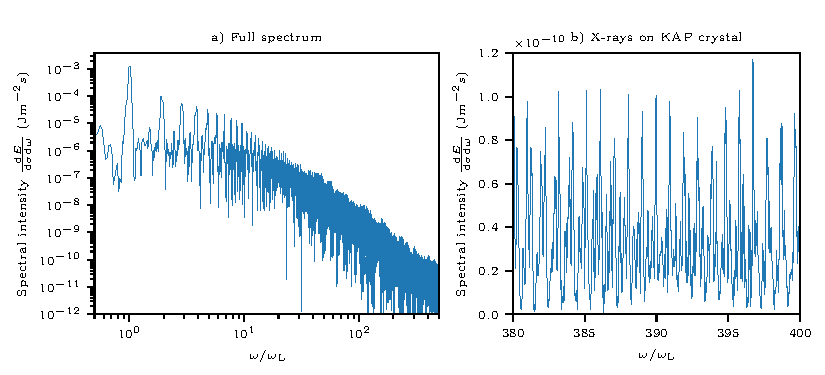
\includegraphics{figures/gemini/gemini_xray_harmonics}
	\caption[XHHG on the GEMINI PW laser system.]{\textbf{1D PIC simulation of XHHG on the GEMINI PW laser system.} The beamline is incident on a SiO$_2$ target under optimised conditions. a) The full harmonic spectrum. b) Window of the spectrum recorded by the KAP OHREX crystal. The harmonics are clearly visible.}
	\label{fig:geminixrayharmonics}
\end{figure}

A parameter scan of \ac{XHHG} as a function of $S$ can be performed by varying the laser intensity, via beam apodisation, and the target material. The majority of shots will use target wheels of the relatively high damage threshold fused silica with the plan to advance to a Kapton tape. The fused silica targets are chemically etched in one corner to aid alignment.
% TODO cite the below
Since HHG is suppressed for circularly polarised light, bremsstrahlung emission and other X-ray production mechanisms can somewhat be ruled out by comparing the \ac{XHHG} signal observed for p- and circularly- polarised light, produced via a quarter wave plate. At \qty{45}{\degree} \ac{AOI}, however, this suppression is not total. And, the efficiency of heating is also reduced, reducing the signal from bremsstrahlung.

The OHREX spectrometer design is such that its technical complexity is entirely bound to the spherically bent OHREX crystals, thus reducing the challenges of alignment \cite{beiersdorferLineshapeSpectroscopyVery2016} and replica building. It is relatively insensitive to the distances between source and crystal (2.4 m) and from crystal to image plane (0.524 m). Indeed, previous experiments deemed unnecessary the adjustment of the bellows to bring the detector to the best focal plane. Variation in the angle of incidence from \qty{38.7}{\degree} shifts the spectral image away from the nominal energy range. 
% TODO am I doing this? The variation is relatively sensitive, for the quartz ($10\bar{1}1$) crystal, a change in energy of \qty{8}{\%} is obtained by a change in angle of \qty{50}{\mu rad} \cite{macdonaldAbsoluteThroughputCalibration2021}. Confirm this with Ed
The alignment of the spherically bent crystal planes to the crystal surface enables the relative convenience of optical alignment. A light source placed at the target location produces a line focus on some tissue paper placed at the focal plane. 

Filtering is necessary to reject the high-intensity low-order harmonics, however, for photon energies in the 600 eV range accessed by the KAP crystal, the standard beryllium filter transmission is too low. 400 nm of aluminium flash-coated onto 1 micron of mylar is more suitable, corresponding to a transmission of \qty{16}{\%} at 600 eV \cite{henkeXRayInteractionsPhotoabsorption1993}. Light leakage and alignment will be checked with IP before switching to the Raptor Photonics Eagle XV in vacuum X-ray CCD camera (EA4240XV-BN-CL) \cite{EagleXVVacuum} to utilise the high shot rate on GEMINI PW. Note that with $2048 \times 2048$ active pixels of size \qty{13.5}{\mu m} $\times$ \qty{13.5}{\mu m}, not all of the 4 cm crystal image can be captured by the camera. The CCD camera must be liquid-cooled. For the prevention of damaging condensation on the camera window, a manual gate valve is required to isolate the OHREX when pumping the main chamber (waiting for the camera to reach acceptable temperatures while under vacuum would be prohibitively long). 

It is essential to check there is the required resolution in both the spectrometer and the CCD camera for harmonic observation. For the highest energy crystal, nominal photon energy of 2.405 keV, 96 harmonics sit in the range accessed by the crystal, corresponding to a fractional energy $\Delta E/E =$ \num{6.45e-4} between harmonics. At  $\Delta E/E =$ \num{1e-4}, the OHREX crystal resolution is sufficient. Characterising the spectral shape of the harmonics at such energies is probably beyond the capability of such a detector. Those 96 harmonics are spread over the 4 cm crystal image. At a resolution of \qty{13.5}{\mu m}, the CCD camera has 31 pixels between harmonics and the harmonic width is about a pixel.

% TODO KAPTON sims
sims:
Running a new SiO2 HHG sim, hopefully, will show that we have a better efficiency than the previous simulation. Then pop that in here.

The optimised conditions of the GEMINI PW system enables access to the ZVP regime. Here, due to the presence of the preplasma, there is significant energy storage in the pseudo-capacitor at the front surface of the plasma that can then be re-emitted during the expansion phase \cite{gonoskovUltrarelativisticNanoplasmonicsRoute2011}. This is reflected in the spectrum of the reflected radiation, the conservation of energy boundary conditions no longer apply and attosecond spikes can be observed even without the presence of a filter.

While ROM does not strictly apply for the optimised theory of the GEMINI PW laser system, the spectrum does not deviate significantly from it. Hole boring theory still applies.

% TODO use simulation intensities instead of ROM calculated ones.


Signals at the detector can be predicted using the theory of Chapter \ref{ch:3-orion} using GEMINI PW parameters. Applying ROM and hole boring theory to a fused silica target and accounting for filtering and assuming no merging of harmonics, one can anticipate signals at the OHREX crystal position of \qty{19.6}{\mu J.sr^{-1}} per harmonic at 0.6 keV for the KAP crystal and \qty{1.89}{\mu J.sr^{-1}} per harmonic at 2.405 keV for the quartz ($10\bar{1}1$) crystal. Orienting the OHREX for s-polarisation, to maximise the signal at the image plane, corresponds to an average of 3.4 photons per pixel and 0.20 photons per pixel respectively. The quantum efficiency of the detector is close to \qty{100}{\%}. These photon numbers are no less than those measured in the ORION experiment while the background will be lower due to the order of magnitude lower energy on target. Implying adequate statistics for the observation of such signals.

% TODO compare these results to the sims: currently sims predict 50 times lower intensity, comment that at least for the KAP crystal we have room to apodized and reduce beam divergence and increase signal so we should get this at least

\section{Observation of ZVP electron bunches}\label{sec:ch4-zvp}
The second stage of the GEMINI PW experiment is the first observation of ZVP electron bunches both mass-limited and bulk-produced. There has been some experimental evidence of attosecond and nano-Coulomb electron bunch generation from nano-targets \cite{cardenasSubcycleDynamicsRelativistic2019,hornyGenerationSingleAttosecond2021} and in reflection from solids \cite{linIsolatedAttosecondElectron2020, thevenetVacuumLaserAcceleration2016} with the latter demonstrating satisfaction of the specific conditions for \ac{VLA} to 10 MeV for a mildly relativistic laser pulse ($a_0 \approx 3.1$). These experiments have guided the planning process for this experiment stage.

This experiment aspires to produce mass-limited ZVP electron bunches in the configuration simulated in Figure \ref{fig:experimentsetuphhgbunches2}. % TODO repeat this simulation with the Silicon wafer target
\begin{figure}
	\centering
	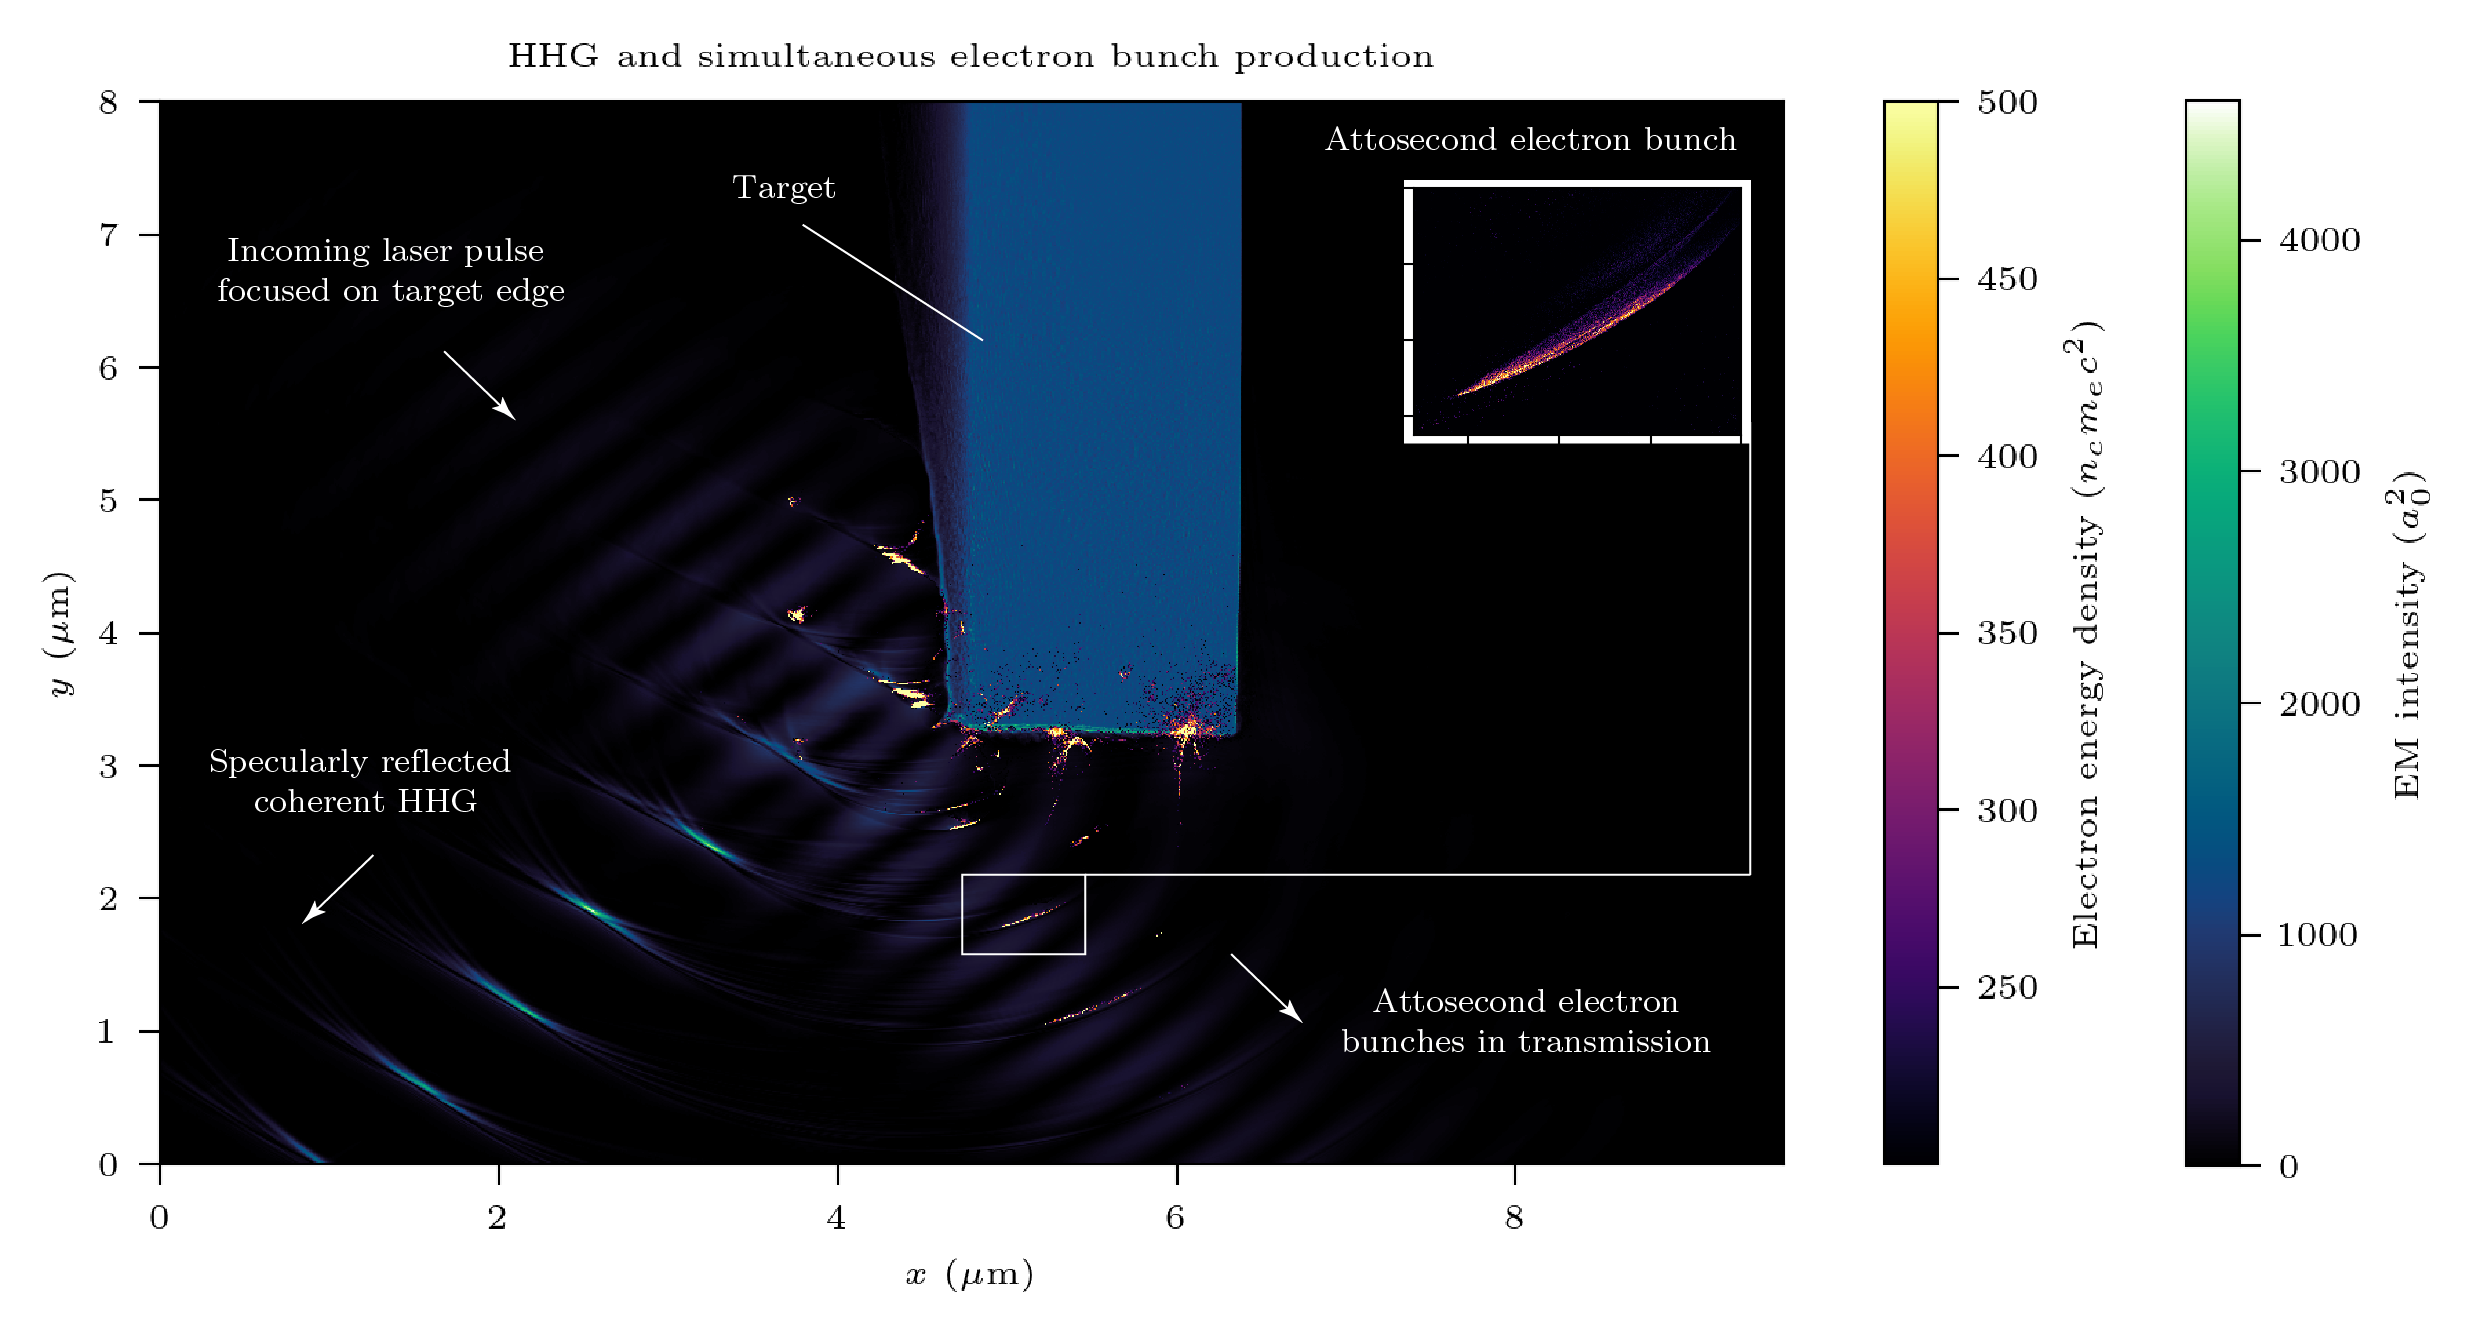
\includegraphics[width=1\linewidth]{figures/zvp/Experiment_setup_HHG_bunches2}
	\caption[Planned GEMINI-PW experimental setup for the measurement of ZVP electron bunches.]{A simulation of the planned GEMINI-PW experimental setup for the measurement of ZVP electron bunches. This novel setup enables the simultaneous measurement of attosecond ZVP electron bunches and their coherent emission of X-ray light. The GEMINI-PW laser pulse is incident at \qty{45}{\degree} on the low-density polyethylene target with a preplasma scale length of $0.2\lambda_\mathrm{L}$. For this angle of incidence, transmitted bunches and specularly reflected X-ray harmonics are produced at a frequency of $\omega_\mathrm{L}$.}
	\label{fig:experimentsetuphhgbunches2}
\end{figure}
Emitted electron bunch energies are maximised by focusing the 2 micron laser spot onto the corner of a transversely mass-limited target. The simulations suggest it is possible to simultaneously measure the specularly reflected \ac{HHG} and the attosecond ZVP electron bunches that produce it. Note via equations \ref{eq:zvp_N} and \ref{eq:zvp_T}, the low-density target of Figure \ref{fig:experimentsetuphhgbunches2} are a more practical choice for the experiment relative to the aluminium targets of predominant use in Chapter \ref{ch:2-zvp}, producing larger and more energetic bunches. Both bulk and mass-limited ZVP electron bunches will be generated. Via conservation of transverse momentum, the two species will be spatially separated at the observation point with bulk bunches at lower energies, experiencing no further acceleration phases post ZVP.

While normal incidence was most convenient for the initial ZVP simulations, oblique incidence is more optimal for \ac{HHG} \cite{gonoskovUltrarelativisticNanoplasmonicsRoute2011, edwardsXRayEmissionEffectiveness2020} and as can be understood from equations \ref{eq:zvp_Tzvp_theta} and \ref{eq:zvp_Uzvp_theta}, the new energy scaling expressions, for the ZVP mechanism. Not only is oblique preferable but it is essential to mitigate damage to the laser optics via back-reflection. The \ac{HHG} beam intensity at the focus can be over 1000 times that of the incident laser pulse \cite{quereReflectingPetawattLasers2021}. It is necessary to conduct PIC code parameter scans for this new geometry.

High target edge precision is essential for the generation of attosecond duration ZVP electron bunches. The CLF Target Fabrication team has created 300 $\mu$m silicon wafer targets via the Bosch process with well-defined edges of sub-micron precision. The target design is presented in Figure \ref{geminisiliconwafer}a.
\begin{figure}
	\centering
	\includegraphics{figures/gemini/gemini_silicon_wafer}
	\caption[Attosecond ZVP electron bunch targets]{\textbf{Targets designed for observation of ZVP electron bunches.} a) Target array design with conical array holder and tapered finger, lengths in mm. b) Scan of the etched wafer, striations develop towards target rear due to etching technique. c) A 3D plot of surface variation. Scalloping and striations are visible but too small to interfere with laser pulse transmission at \qty{45}{\degree}. d) Lineouts of c), the $y$-profile is along the target edge of interest.}
	\label{fig:geminisiliconwafer}
\end{figure}
The tapered finger structure adds a failure point to mitigate damage to adjacent targets via shock propagation. The cone of the array holder is of sufficient size for the full laser pulse to access the target edge. Scans, detailed in Figure \ref{fig:geminisiliconwafer}, found an average surface roughness of \qty{74.4}{nm}. The etching technique leads to scalloping of the surface parallel to the target surface and perpendicular striations towards the target rear. Neither pose any concern with regards to interfering with the laser pulse in transmission. The target design and scans were performed by Sam Astbury \cite{astburyTargetFabricationGroup2024}. Before firing target edges, HHG production will be optimised for unstructured silicon wafer targets, providing information on the bulk propagating ZVP electron bunches for comparison with the mass-limited case. Again, a quarter-wave plate can be implemented to suppress the ZVP mechanism in the absence of vector potential zeroes.

Some relaxation can be anticipated in the requirement for sub-micron precision. There will be some target smoothing via preplasma expansion and the smoothing effect of the main pulse interaction as noted by Dromey \textit{et al} \cite{dromeyDiffractionlimitedPerformanceFocusing2009}. Furthermore, transmission direction is dictated by laser vector potential and not surface angle, unlike reflection. At worst, ZVP energy scalings will be mildly affected by the change in angle. Thus tape drives will also be explored as an option. However, the \qty{50}{\mu m} jitter of such devices suggests a success rate of $\sim$ 4 \%. The gathering of sufficient statistics is not necessarily unreasonable with the high shot rate of GEMINI PW. Shot-to-shot variations in laser pulse focal spot position are typically on the order of the focal spot itself. It is likely therefore that a third of silicon wafer target shots will hit a adequate portion of the target edge. 

Successful shots will be identified using a third harmonic imaging line \cite{dromeyThirdHarmonicOrder2009}. This diagnostic will also reduce the uncertainty of the hole boring calculations. The non-linearity of the third harmonic production mechanism reduces the possibility of background noise, producing a clear signal and a closer match to the true spot size than the X-ray emission diagnostics of the ORION experiment. For high resolution, the collimating reflective optic must be placed roughly the distance of the $f/2$ parabola focal length from the main interaction. Near the main interaction region, the B-integral is large thus precluding the use of ND filters and lenses. Instead, a wedge, typically double-passed acts as an attenuator to extract the lower order highly divergent harmonics. A hole allows the less divergent higher orders through, enabling on-shot measurement. Far from the interaction, the collimated third harmonic signal can be extracted, filtered, refocused and imaged. Some light is reflected to the target via the wedge on the second pass, however this is not a concern. The focal length of the new optic is larger than that of the $f/2$ parabola and path lengths are on the order of a nanometre at which time the target does not reflect specularly. 

Resolving the \qty{16}{\mu m} GEMINI PW spot is significantly more challenging than the \qty{6}{\mu m} spot of the 1 J Astra-GEMINI laser system. This imaging line has been modelled by the ORION laser scientists using Zemax \cite{AnsysZemaxOpticStudio} accounting for all diffraction and spherical aberration. They have identified a set-up using two spherical mirrors for collimated and imaging that provides \qty{10}{\mu m} resolution with 20 times magnification, reasonably resolving the spot. While the high spatial orders associated with the clipping of the reflected beam at the target edge cannot be resolved, this should significantly alter the image structure, enough to identify their presence. Over time the wedge will be coated by material ablated from the main target interaction and will need to be replaced to prevent absorption increases and corresponding heat damage.

The size of the wedge hole must be established. Sitting somewhere between the near and far field, to first order, rays from all parts of the spot are lost equally through the hole in the wedge. After passing through the optical system, therefore, the wedge hole should simply reduce the signal at the image plane and not affect the resolution but should be modelled. One could argue that the wedge can reduce the spherical aberration by the removal of paraxial rays. The larger the hole the less likely the clipping of the potentially highly divergent high harmonic beam. Eventually this will impact the third harmonic image resolution. At a minimum the OHREX crystal must be fully illuminated requiring a half angle of \qty{0.71}{\degree}.
%TODO decribe B integral

%TODO double-check these numbers
Applying the extended ZVP theory to the oblique incidence case for GEMINI PW parameters predicts electron bunches with a charge of $\approx$10 nC and energy of $\approx$30 MeV. Thus, a \qty{15}{\mu m} of aluminium foil filter will reject the laser light without significantly affecting the electron bunches.
% TODO calculate the angle of electron bunch and divergence in a sim
Firstly, mass-limited and bulk electron bunch trajectories and beam divergences will be imaged on a LANEX screen. An MeV electron spectrometer aligned to the target edge can then measure the time-integrated energy spectrum. The spatially separated bunch types can be independently measured by adjusting the spectrometer position. Mordovanakis \textit{et al} used Image Plate stacks to obtain the electron bunch structure and emission angle. This may prove necessary if the bunch types overlap due to high divergence \cite{mordovanakisQuasimonoenergeticElectronBeams2009}. 

While resolving attosecond durations remains a serious technical challenge of experimental science, we hope to measure the production of Coherent Transition Radiation from a secondary target and therefore infer the presence of a bunch train \cite{linIsolatedAttosecondElectron2020}. 


COTR - awaiting papers from Peter

When electrons pass from one medium to another they emit transition radiation, in this case, the aluminium filter. If they are arranged into temporally regular spaced bunches that radiation becomes coherent and harmonics of the temporal spacing of the bunches can be observed. Both bulk propagating and mass-limited ZVP electron bunches will produce COTR, however, the attosecond duration should mean the mass-limited bunches produce significantly brighter COTR that extends to XUV energies but that can be distinguished even at the optical range.


% TODO add somewhere: Note that in the absence of attosecond resolution diagnostics, measuring the harmonic spectrum of the coherent \ac{HHG} is the only way to reconstruct the temporal shape of the pulse. Simulations have suggested that the reflected spectrum produced by Coherent Synchrotron Emission of the electron bunches is approximately Fourier-limited \cite{cousensElectronTrajectoriesAssociated2020}.

% here with the edits
\section{Application of HHG to white light Laue diffraction}\label{sec:ch4-laue}
The eventual but still somewhat distant goal is the generation of an attosecond X-ray diagnostic to illuminate crystal dynamics on attosecond timescales. Inspired by Laue diffraction measurements demonstrating dislocation microstructure of shocked crystals \cite{suggitNanosecondWhitelightLaue2012}, this will be a proof of principle test of Laue diffraction from an X-ray harmonic beam of a single unshocked crystal.

It was Laue diffraction that led to the discovery of Bragg's law,
\begin{equation}\label{eq:gemini-braggs_law}
	n\lambda = 2d\sin\theta
\end{equation}
for diffraction order, $n$, incident wavelength, $\lambda$, the distance between crystal planes, $d$, and angle between the crystal plane and the incident photon, $\theta$ \cite{braggDiffractionWaves1915}. Irradiation of a crystal target with a `white light', \textit{i.e. } a broadband X-ray source, Equation \ref{eq:gemini-braggs_law} is satisfied for a range of crystal planes and corresponding angles simultaneously, \textit{producing Laue spots} accordingly. The quasi-broadband X-ray harmonic beam is well suited to such an experiment provided sufficient photon numbers can be obtained.

This will be attempted using the \ac{BBXRD} diagnostic placed in the path of the specularly reflected beam and roughly 50 cm from the target. The lead-shielded and IP lined BBXRD contains the crystal sample with a hole to allow the harmonic beam to enter. The sample is placed at an angle on a rotatable washer enabling a range of angles and corresponding energies to be tested: starting with a quartz target to investigate photon energies of 1.7 - 2.5 keV and moving to silicon to explore energies of 2.4 - 3.3 keV. The IP must be shielded to reject laser light, beryllium is most suitable. It may be necessary to integrate over multiple shots to produce the Laue spot.

\section{Contrast}\label{sec:ch4-contrast}


\subsection{Contrast on GEMINI PW}
% Observation of the ZVP mechanism and HHG production requires a sufficiently steep density gradient at the laser-plasma interface. An inevitable challenge of \ac{CPA} laser systems is the existence of prepulses that heat targets, causing them to expand significantly before the arrival of the main pulse. To increase the laser contrast, to the point where there is no preplasma formation, GEMINI-PW utilises a Double Plasma Mirror setup prior to the main interaction \cite{doumyCompleteCharacterizationPlasma2004}. Investigation of preplasma generation will occur in parallel to the main experimental goals.

An underlying current of this thesis has been the subject of prepulse and corresponding preplasma expansion. While bright X-ray harmonics have been observed on both the Vulcan \cite{dromeyBrightMultikeVHarmonic2007} and ORION sub-ps laser systems, few cycles laser pulse systems routinely underperform. To date only at normal incidence (thus minimising heating) have harmonics been observed on GEMINI PW \cite{dromeyCoherentSynchrotronEmission2013}. Evidence points to preplasma formation. The only parameter that has been shown to suppress HHG from a p-polarised relativistic laser pulse is an overlarge preplasma \cite{dollarScalingHighorderHarmonic2013} and indeed the transition to suppression is rapid \cite{kahalyDirectObservationDensityGradient2013}. While there exists established theories on the operation of plasma mirrors, these are based on fairly large assumptions that remain untested. Given the notoriety of the challenge of observing SHHG despite laser contrast being a relatively well understood concept and the general successes attributed to hydrodynamic codes, it seems quite possible that these large assumptions are the critical concern. They could also be responsible for the range of optimal scale lengths observed in experiments. 

The last available contrast measurements of the GEMINI PW laser are presented in Figure \ref{fig:geminicontrast}. 
\begin{figure}
	\centering
	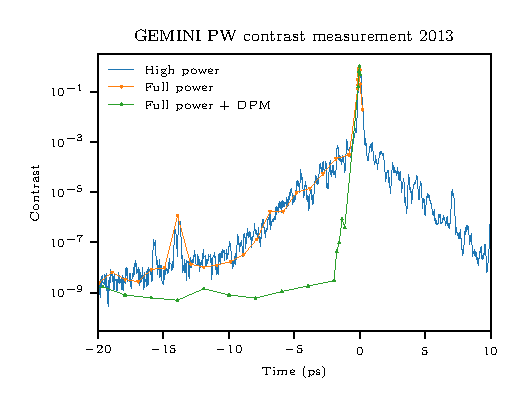
\includegraphics{figures/gemini/gemini_contrast}
	\caption[Native contrast of the GEMINI PW laser system.]{Native contrast of the GEMINI PW laser system measured using the Sequoia third order autocorrelator scans. The noise floor of the detector is $\approx 1\times 10^{-9}$. The resolution is 100 fs, thus the main pulse is not resolved by the detector.}
	\label{fig:geminicontrast}
\end{figure}
The \ac{DPM} setup improves the contrast by at least $10^5$. More recent measurements of the GEMINI PW DPM system have found a reflectivity of \qty{1.23e-4}{\%} and \qty{60}{\%} before and after switch on, corresponding to a contrast enhancement of \num{4.88e5}. Note that the DPM setup includes an acetate debris shield, without which shot quality would quickly degrade from plasma ablation between the mirrors.


% TODO includes a plot of preplasma from HYADES.
Note in Figure \ref{fig:geminicontrast} the early switch-on of the plasma mirror system. For a peak intensity on \ac{PM} of \qty{1e16}{W.cm^{-2}}, this switch occurs an order of magnitude below typical ionising intensities \cite{umstadterRelativisticLaserPlasma2003}. Early PM switch-ons is nothing new \cite{caiTimeresolvedMeasurementsReflectivity2009}, however, it points to a serious issue. Such early switch-ons cannot be described by the basic theory nor hydrodynamic simulation. Perhaps all can be explained by the complex atomic scale interaction of the laser pulse with the dielectric AR coating. Indeed, perhaps the haste to maximise the contrast at the nanosecond pedestal has been the downfall at the picosecond scale. And yet, providing the measured GEMINI PW contrast data to HYADES simulations predicts acceptable preplasmas, inconsistent with the experiment results. 

Recent work has shown evidence of the propagation of an opacity front into a target due to laser prepulse before ionisation and plasma formation. Such a transition from transparency will dramatically affect laser pulse energy deposition into the target leading to significantly earlier plasma mirror switch-on times. The interaction appears to occur a few picoseconds, a timescale to which preplasma scale length is highly sensitive. Note that such an interaction would be impossible to simulate given the multiple scales upon which preplasma formation occurs and the complexity of the transition to opacity. The GEMINI experiment, however, provides an excellent opportunity to probe this process in parallel to the main experimental goals.

 A pure fused silica target consists of valence and conduction bands only. Electrons are excited to the conduction band by the laser and then simply drop back down again. As impurities are added to the target, the band structure becomes more complex and electrons can drop to intermediate states from which they cannot then return easily to the ground state. Thus, more energy can be absorbed and the transition to opacity occurs at earlier times. Hence, the more pure a silica target, the later the transition to opacity and the smaller the preplasma scale length. This also suggests switching out the first plasma mirror for a pure uncoated silica target could also improve contrast at the timescales where it matters. Now the first PM deals with the ps pedestal with its later switch on and the second PM the ns pedestal with its AR coating.

Presumably early plasma formation also occurs for Vulcan or ORION targets, however, once relativistic intensities are reached, recompression will occur. For such long pulse durations, there is sufficient time for steepening before the main interaction. 

Contrast reduction will only become more critical with the arrival of sub-eta watt class next generation laser facilities where native picosecond pedestals will already be relativistic. Steep preplasma scale lengths is not only relevant to the matters presented in this thesis but is essential for any thin foil interaction including the popular use case of ion acceleration via TNSA.

To investigate early plasma switch on, a \qty{50}{ps} chirped probe beam will be focused on the target. Optical spectrometers in transmission and reflection will identify the opacity and plasma generation times respectively. This measurement could categorically demonstrate the failure of hydrodynamic codes for any pre-ionisation laser pulse intensities. One may wonder why such a failure is not identified in other branches of HED physics, such as the case of Inertial Confinement Fusion. It is simply a matter of scales. These effects are only relevant for the few femtosecond petawatt laser systems in this case of high sensitivity to preplasma scale length.
% TODO look into cold opacity in hydro code
To distinguish the probe beam from the bright non-linear target interaction, it will be focused on the interaction area out of the main interaction plane and with opposite polarisation.

\subsubsection{Strategy}
A series of contingencies has been developed to ensure the observation of harmonics under the assumption that preplasma scale length is the main issue. Phases increase in cost to peak laser intensity and therefore to the theoretical harmonic limit. During optimisation, the OHREX will be replaced with an XUV spectrometer since only the lowest orders will be visible. As of 2019, no experiment to confirm HB theory had been performed on a PW system \cite{vincentiAchievingExtremeLight2019}. Such UV spectrometer measurements could be very interesting both to confirm the HB theory in the PW regime and to infer the intensity increase at PM focus. The first step will be to scan through the focal spot of the laser. Wavefront curvature at the target from slight defocussing can reduce divergence from hole boring thus increasing intensity levels at the detector while also reducing pre-heating. 

The next action will be to apodise the beam, again this reduces the intensity on target and the harmonic beam divergence and has been shown to tip preplasma scale length into the optimal regime for HHG \cite{kahalyDirectObservationDensityGradient2013}. This will reduce the intrinsic prepulse intensity by the same factor as the main pulse. To ensure the SHHG roll-off is above the 2.4 keV harmonics (such that the signal on OHREX is non-negligible), requires $a_0 > 8$. Such apodisation would reduce the prepulse by $\approx$ 10 times. Corresponding a reduction in the beam radius of a factor of 2. Apodising can also help remove higher spatial orders, improving the spot at focus. While harmonics were observed on the 1 J precursor to GEMINI PW, Astra-Gemini, apodising back to Astra-Gemini parameters does not guarantee success, the new front end procudes a unique prepulse profile.

The intensity on DPM can be reduced leading to later switch-on times but a lower peak reflectivity. Failing that, there are more drastic measures available. First, a second target chamber layout has been designed that will reduce the angle of incidence on target to \qty{30}{\degree} to reduce target heating and second, frequency doubling is known to significantly enhance contrast. In fact, as with ORION this will likely overshoot, producing effectively zero preplasma.

Testing frequency doubling would be very useful for demonstrating the validity of the new contrast theory. The frequency doubling crystal available at GEMINI PW will reduce the intensity on target both from the generation efficiency (\qty{25}{\%}) and apodisation (\qty{9}{\%}) (the crystal has a diameter of 60 mm), therefore if there is an improvement in signal, it must be from the improvement to contrast. While Kahaly \textit{et al} were able to observe harmonics for a beam apodised to $a_0 = 0.7$ provided the scale length was optimised, resorting to this method to produce harmonics would preclude the observation of X-ray harmonics ,however, it would justify the investment into a larger frequency doubling crystal for future HHG experiments at GEMINI PW. Such a setup would not require a DPM and the diffraction limited spot is smaller. Hence, despite the inevitability of efficiency cost due to the frequency doubling process, similar intensities on target could be realised provided a 25 \% efficiency non-apodising frequency doubling crystal.

Once harmonics are visible, aspects of the system can be changed and the opacity and early switch-on hypotheses can be tested by looking for quantitative improvements to the signal. Replacing the pure fused silica target with impure BK7 or AR-coated targets should reduce the harmonic signal. Equally, replacing the first PM in the DPM chain with an uncoated PM should delay the PM switch on and improve the signal. Note that the CWE signal is distinguishable from the HHG signal: it is more divergence and experiences a sharp cuts off at the plasma frequency \cite{kahalyDirectObservationDensityGradient2013}.

\subsection{Kahaly mirror}
At some point, the signal will overshoot and enter the CWE regime, preferably early in the list of contingencies presented, and the preplasma scale length can now be optimised. Kahaly \textit{et al} \cite{kahalyDirectObservationDensityGradient2013} designed a simple but elegant method to do this. Simply partially cover a mirror in the laser chain with a small mirror. The difference in path length of light on this mirror is determined by the mirror thickness and distance from the main laser mirror surface. Thus this added prepulse arrival time at the target can be controlled. Since this has effectively apodised the beam, the parabola will then focus the prepulse spot to a larger area compared to the main pulse spot ensuring a uniform preplasma across the main spot while the diffraction-limited main spot will experience minimal aberration from to the subtracted prepulse. The target must be routinely monitored to ensure the prepulse spot coincides with the main pulse spot. The mirror should have a mirrored back surface and an AR-coated front surface with a slight angle between the two faces to prevent any parasitic prepulse.

Kahaly \textit{et al} show a linear relationship between main pulse delay relative to prepulse and scale length (due to more time for the preplasma to expand) but also note that for the same scale length, a larger delay (accompanied by smaller energy in the prepulse) produces higher quality harmonics. This could be understood as a natural consequence of the lower plasma temperatures, which improve the ability of the system to perform coherent SHHG behaviour. If harmonics are accessed using the Kahaly method, the signal can be improved our signal by moving the prepulse mirror further from the main pulse mirror while also reducing the fraction of overlap between the two mirrors to reduce the energy in the prepulse. The Kahaly mirror should be placed before the final mirror before the parabola. The further back in the chain it is placed, diffraction from the mount can cause greater danger to the optical system. The linear relationship between main pulse delay and scale length coupled with the XUV HHG signal measurements can be applied to discrete changes to the system to quantify contrast improvements.


\section{Summary}
This chapter has detailed the strategy, goals and hypotheses surrounding the upcoming GEMINI PW experiment, including supporting PIC and hydrodynamic simulations. It may prove that the contrast of GEMINI is insufficient to enable access to the highly interesting regime of SHHG. However, should this be the case a strong plan of action has been laid out that should both enable some level of success in harmonic generation and provide invaluable insights that could change the approach to SHHG experiments in the future. If harmonics can be resolved, there are many exciting avenues for new physics. Namely, the main experimental goals are the resolution of X-ray harmonics, the observation of ZVP electron bunches, the application of the harmonic beam as a diagnostic tool and the measurement of attosecond chirp on optical and XUV harmonics.

% TODO PIC sims heating effect
%TODO add a comment about the use of HHG as a heating source, highly efficient highly penetrating
% TODO hyades (hmm no maybe PIC? but then cant do heating effect.. can use heaths code for tempeerature in smilei) sim of ORION hhg beam entering a plasma and heating vs ORION laser.
% TODO hyper spectral imaging

% TODO CHECK IN THE TARGETS LIST THERE IS ALSO SIMPLE SILICON WAFER UNSTRUCTURED TARGETS

% TODO discuss CSE theory and modified thing and optimised scale length and show pic of pulse structure
